% !TEX TS-program = pdflatex
% !TEX encoding = UTF-8 Unicode

% This is a simple template for a LaTeX document using the "article" class.
% See "book", "report", "letter" for other types of document.

\documentclass[11pt]{article} % use larger type; default would be 10pt

\usepackage[utf8]{inputenc} % set input encoding (not needed with XeLaTeX)

%%% Examples of Article customizations
% These packages are optional, depending whether you want the features they provide.
% See the LaTeX Companion or other references for full information.

%%% PAGE DIMENSIONS
\usepackage{geometry} % to change the page dimensions
\geometry{a4paper} % or letterpaper (US) or a5paper or....
% \geometry{margins=2in} % for example, change the margins to 2 inches all round
% \geometry{landscape} % set up the page for landscape
%   read geometry.pdf for detailed page layout information

%%% Line Spacing
\usepackage{setspace}
\onehalfspacing

\usepackage{graphicx} % support the \includegraphics command and options

% \usepackage[parfill]{parskip} % Activate to begin paragraphs with an empty line rather than an indent

%%% PACKAGES
\usepackage{booktabs} % for much better looking tables
\usepackage{array} % for better arrays (eg matrices) in maths
\usepackage{verbatim} % adds environment for commenting out blocks of text & for better verbatim
\usepackage{subfig} % make it possible to include more than one captioned figure/table in a single float
\usepackage{amsmath, amssymb, amsthm, lastpage}
% These packages are all incorporated in the memoir class to one degree or another...

%%% HEADERS & FOOTERS
\usepackage{fancyhdr} % This should be set AFTER setting up the page geometry
\pagestyle{fancy} % options: empty , plain , fancy
\renewcommand{\headrulewidth}{0pt} % customise the layout...
\lhead{Team \# 16677}\chead{}\rhead{Page \thepage\ of \pageref{LastPage}}
\lfoot{}\rfoot{}\cfoot{}

%%% SECTION TITLE APPEARANCE
%\usepackage{sectsty}
%\allsectionsfont{\sffamily\mdseries\upshape} % (See the fntguide.pdf for font help)
% (This matches ConTeXt defaults)

%%% ToC (table of contents) APPEARANCE
%\usepackage[nottoc,notlof,notlot]{tocbibind} % Put the bibliography in the ToC
%\usepackage[titles,subfigure]{tocloft} % Alter the style of the Table of Contents
%\renewcommand{\cftsecfont}{\rmfamily\mdseries\upshape}
%\renewcommand{\cftsecpagefont}{\rmfamily\mdseries\upshape} % No bold!

%%% END Article customizations

%%% The "real" document content comes below...
%\date{}

\begin{document}
\begin{titlepage}
    \vspace*{\fill}
    \begin{center}
      \Huge{Rapid Scheduling: A Constraint Satisfaction
        Approach to River Usage}\\[0.5cm]
      \Large{Team: 16677}\\[0.4cm]
      \today
    \end{center}
    \vspace*{\fill}
  \end{titlepage}
\newpage
\vspace*{\fill}
\tableofcontents
\vspace*{\fill}
\newpage

\section{Preliminaries}
\label{sec:prelims}
%Possibly include some comparisons of our model to existing research if any.

\subsection{Introduction}
\label{sec:intro}
Floating down a river is easy enough, but imagine scheduling an entire
season of rafting trips for hundreds of people.  A \textit{scheduling problem}
occurs when there are start and end times and start and end locations for a group of people
or objects. The schedules of the group must be arranged such that all
participants start and stop as desired. Between the start and stop, they
must follow any rules stated in the problem.

We consider a scheduling problem for the Big Long River with visitors who desire to
raft down it. The goal is to schedule as many visitors as possible in a six
month season.  Visitors depart from First Launch and finish at Final Exit,
225 miles downstream. They are seeking a relaxing and authentic experience and
will become dissatisfied if they do not receive one. While scheduling
dissatisfied visitors is allowed, we seek to schedule them so as many
visitors are as satisfied as possible.


\subsection{Definitions and Terminology}
\label{sec:defs}
% CSP a group of generally NP-hard problems.
% travel group
% itinerary
% NP-hard
% big O
% river length = L
% days in the season = S
% happiness as satisfaction: related to encounters and actual trip speed
% tolerance: brief description plus see section blah
% carrying capacity
\begin{itemize}
\item Big O: (of an algorithm) Also ``complexity.'' A function relating the
time it takes to solve a problem and the inputs of the problem. For instance,
a function whose Big O is O(x) computes in linear time.

\item Carrying Capacity: The amount of visitors a river can see in a single
year, while maintaining the likelihood that all visitors will be scheduled and
remain satisfied.

\item Constraint Satisfaction Problem (CSP): A type of problem solved by
assigning values to variables. These values must be within specified domains.
The problem is solved when all variables have values within the specified
domains -- e.g. they have values that satisfy all constraints.

\item Group: See ``visitor.''

\item Itinerary: The ordered list of campsites a visitor will stay at each
night.

\item Non-deterministic Polynomial-Time Hard Problem (NP-hard): A class of
problems whose solutions, if they exist, behave unpredictably, and are
provable in polynomial time -- see ``Big O.'' Constraint Satisfaction Problems
are a type of NP-hard problem.

\item Visitor: Also ``group.'' A person or a group of people
seeking to travel the Big Long River by raft. Their raft could be powered
by oar, or it could be motorized. Visitors are very irritable and will
become unhappy if they see other visitors, don't get their desired water
time each day, or don't get scheduled.

\item Satisfaction: (of a visitor) Visitors seeking to raft the Big Long River
start with a satisfaction of 100. This number will drop each time the visitor
passes or is passed by another visitor, or doesn't get their desired water time 
(too much or too little of it) each day. It is possible for a visitor's 
satisfaction to drop to zero by these two factors alone. Visitors who are not 
able to be scheduled have a satisfaction of zero.

\item Season: A six month season is assumed to have 180 days; that is,
six months times an average of 30 days per month.

\item Success Rate: The likelihood a season will have a valid schedule
given certain parameters.

\item Tolerance: The amount of campsites a visitor's travel plan can be
altered by. For instance, a tolerance of 1 would allow a visitor desiring
to move four campsites each day to move between three and five campsites
each day. This is done in order to accommodate for other visitors who may
be in the desired spot.

\item Water Time: Visitors specify how much time they want to spend on the
water each day. This value is the same for each day of the trip. A visitor's
satisfaction rating will drop if they are forced to spend
more or less than this amount of time on the water.

\item X: The current number of trips taken by visitors down the Big Long River
each year.

\item Y: The number of campsites on the Big Long River. Unless otherwise stated,
this was assumed to be 128, as provided by literature\cite{NumCampsites}.
\end{itemize}

\subsection{Assumptions and Simplifications}
\label{sec:assumptions}
% season length
% days traveled opposed to nights
% groups
% encounters
% happiness calculation as satisfaction (show equations)
\begin{itemize}
\item Season Length: A six month season is assumed to have 180 days; that is,
six months times an average of 30 days per month.  Seasons are consistent,
i.e. there exist no peak visitation months or months of higher river flow.

\item Trips ranging from ``6 to 18 nights of camping on the river, start to
finish'' are assumed to allow
between 7 and 19 days of travel on the river, start to finish.

\item Visitors or groups of visitors travel at a constant speed throughout the
trip.  We define this speed by the type of boat they use.  Oar-powered
rubber rafts travel at 4 mph, and motorized boats travel at 8 mph.

\item No visitor separates into more than one group or combines with other
groups during the trip.

\item ``Contact with other groups of boats on the river'' is only counted if
one group passes another group or is passed by another group.

\item Groups are capable of passing one another at any point (i.e. passing is
not restricted by the width of the river or anything else at any time).

\item Visitors specify only their starting date, boat type, and water time,
and only valid values for these parameters. Therefore: They may not start
before the start of the season or so close to the end of the season it
would be impossible for them to finish; they may not have a water time
such that their trip takes less than 7 or longer than 19 days; they may
only choose an oar-powered rubber raft or a motorized boat.

\item Visitors follow the schedule given to them exactly:
no backtracking, skipping.
\end{itemize}


\section{The Solution}
\label{sec:model-details}
Our solution is structured to solve constraint satisfaction problems,
specifically of a scheduling nature.  Our working definition for such a
problem follows: given variables ($X$), values ($D$),
and constraints ($C$), find an assignment of value(s) in $D$
for each $X$ such that all constraints in $C$ are satisfied.  Generally
speaking, a CSP may be defined as a set $(X,D,C)$.
A good example of a CSP is any map coloring problem\cite{DynamicCSP}.

We view the problem of scheduling rafting trips as a progressive and dynamic
CSP. Each day is a constraint satisfaction problem dependent upon the
solution to the previous day's problem.  By limiting the values any variable
may take on and applying efficient algorithms, the CSP becomes tractable.
This allows us to successfully schedule river trips without the need of 
unreasonable computing power.

\subsection{Constraint Satisfaction}
\label{sec:csp}
%variables, values, constraints (rules from problem statement)
%travel groups as variables
%campsites as values
%constraints

Consider that there are exponentially
many combinations of  visitors to campsites during a season.  Many of
these combinations, however, are invalid since no two
 visitors may stay at the same campsite on the same day.
This is an $n-ary$ constraint: a constraint relating $n$ variables.  This sort 
of complexity often causes problems to become computationally intractable.  We, 
however, simply pair all campers and detect collisions at any campsite at the 
current scheduled day
($O(n^2)$ with $n$ as number of  visitors).  This small simplification reduces 
the problem to relatively few constraints.

Each visitor is considered to be a variable
in the CSP and campsites are considered the values.  The domain of
each visitor's values varies day to day as the visitor travels through the
campsites.  Travel distance is derived from
a visitor's average speed of 4 or 8 mph, $v$,  multiplied with a uniformly distributed
random variable for water time, $t$.  This variable must allow the visitor to complete the trip
within 7-19 days. The following equations explicitly
describe these relationships:
$$v*t=OptimalDayDistance$$
$$v*t*7\geq L$$
We ensure generated visitors are reasonably
parameterized to finish a trip on time.  Each visitor is assigned a random
uniformly distributed day for departure, $dDay$, such that
$$v*t*7+dDay\leq S$$
A visitor's maximum travel speed will allow them to finish before
the close of the season.

Visitors are generated en masse using uniformly distributed
variables.  It is possible to load a file containing visitor information
so the program will work on problems of natural rather than simulated
origin.  Once visitors are generated and basic parameters
are set (discussed in \textbf{Section \ref{sec:high-params}}) the program begins
attempting a solution through our solver.

\subsubsection{Backtracking Search}
In order to solve a CSP, one must navigate many combinations
for variables and values. Backtracking search algorithms are often used
to assign values to variables\cite{AI-Intro}.  We use such an algorithm to
assign campsites to our  visitors on a daily basis.
On any given day
$d$, the solver looks to see which visitors are set to depart that day and
adds them to a list, $toDepart$.  Then, all visitors left on the
river from the previous day are added to $toDepart$.  This creates a list of all
 visitors requiring movement for day $d$.  In order to determine
appropriate movements, visitors are assigned campsites one-by-one.  Travel
between campsites is analagous to
distance traveled for the day.  Following
a visitor-campsite pairing, the day's assignments are checked to see if this pairing is
consistent.  If the pairing doesn't conflict with
existing pairings, it is permanently added to the day's assignments.
We then proceed to the next visitor.

When pairings fail, the algorithm attempts new pairings
until success is achieved or no more pairings exist. The entire process is 
structured as a
depth-first-search. When a day's assignment is complete, the algorithm creates
a new CSP for the next day and executes again.  \textbf{Figure~\ref{fig:searchExample}}
highlights the major steps
involved in this process with a simple example.  The algorithm begins by
assigning site $1$ to visitor $A$, denoted
by the diamond below and to the left of the tree-top.  Assigning
site $1$ to $B$ is tried but found to fail.  Instead the algorithm assigns site
$2$ to $B$ (rightmost circle).  At this point, the day would ``end'' and
the algorithm would begin scheduling the next day.  In the event
the next day fails, the algorithm returns to a previous level, as
seen in the example.  In this case, the previous level is the previous day.

\begin{figure}[h]
  \centering
  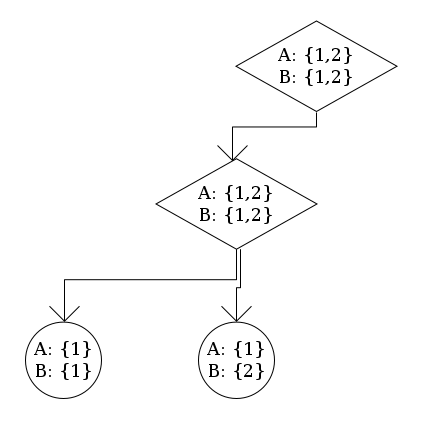
\includegraphics[scale=0.5]{imgs/searchExample.png}
  \caption{An example of the backtracking algorithm's attempt to schedule
     visitors $A$ and $B$ with campsites $1$ and $2$.}
  \label{fig:searchExample}
\end{figure}

Our solver seeks maximal satisfaction of the travelers.
That is, the possible campsites a visitor may travel to are presented to the
solver in order of ideal travel distance.  While not every visitor is guaranteed
to travel their desired distance, the algorithm attempts to satisfy it.

We also calculate the number of encounters
between visitors.  After the itineraries are created, each visitor's campsite
listing is checked to determine how many visitors passed and were passed by
this specific visitor.  By combining the amount of variation from ideal travel distance
and encounters with other visitors, we obtain the total effect on
satisfaction.  The solver relies heavily on several
parameters to relax the problem, making solutions more attainable.

\subsection{Usage of High-Level Parameters}
\label{sec:high-params}
% visitor size
% river length (maybe)
% days in the season
% number of sites
Many values tend to be static.  These include river length, number of days in
the season, and number of campsites.  While each of these values is capable of
drastically affecting the outcome of a given attempt, this effect is limited
by a well-defined range (see \textbf{Section \ref{sec:assumptions}}).  There
are likely optimal values, but finding these would likely place our
problem into the realm of intractable problems.  In an attempt to capture
the complexity of this system, we have introduced a unique variable, $tolerance$.

$Tolerance$ is designed to create a
range for the distance a  visitor may travel in a given day.  This variable
is straightforward at the outset but provides several neat nuances for additional
complexity in the solution.  The introduction of a value range allows
for a larger domain of solutions and variability.  We desire such flexibility
to account for the real-world uncertainty of
directing human beings.  Tolerance extends as an
aggregate for many of the instances where we might expect variability
---such as inclement weather, cancellations, or slow  visitors---
without having to introduce additional parameters.  Tolerance is a
satisfying opportunistic variable for allowing more visitors to be
scheduled.  It allows for the rafting season to be enjoyed by more individuals.

It is important to note a lack of tolerance often creates
problems with no solutions. With visitors locked between one of two
travel distances, scheduling becomes virtually impossible for all but the
smallest number of visitors.



\section{Predictions and Analysis}
% address all of our graphs
% address the question of how to mix the visitors (i.e. oar versus motorized)
\subsection{General Expectations}
\label{sec:expectations}
Before creating the model we developed a few ``common sense'' expectations of
the results.
\begin{itemize}
\item Increasing the visitor size
would make it harder to schedule each visitor at the desired time. The more
visitors one is trying to schedule, the faster the schedule fills up.

\item As the number of visitors on the river during a season increases, it
becomes increasingly likely visitors will pass each other. Passing
is a necessity if the visitors are traveling at different daily
speeds.  Consider a visitor with a daily speed of 8 mph leaving a few days
after a visitor traveling at 4 mph.

\item As tolerance increases, so will the ease of scheduling each visitor. The
greater the tolerance, the greater the likelihood of finding a site to stay
at if other visitors are also in the area.

\item An increase in tolerance will cause a decrease in overall happiness.
An increase in tolerance will allow visitors to travel less than or more
than their desired time each day. Thus decreasing their overall satisfaction.
%WE GOT TO USE THUS!!!!!

\item Assigning more visitors to motor boats (those that travel
at 8mph) will increase the success rate. Visitors that travel faster will
spend fewer days on the river, leaving more space for other visitors.

\item Seasons with less variability in visitor speeds (e.g. seasons where
all visitors travel at 4mph, or where all visitors travel at 8mph) will result
in greater satisfaction. Visitors traveling at the same speed are less likely
to pass each other or to want to stay at the same campsite on the same night.
Greater variation in group speeds will increase the frequency of these
conflicts.
\end{itemize}

\subsection{Results}
\label{sec:results}
The following discusses various results from repeated simulations of our
model.  Each major variable is addressed, but major conclusions are saved for
later (beginning in \textbf{Section \ref{sec:capacity}})

The results of the model tended to be in line with our
expectations (\textbf{Section \ref{sec:expectations}}), especially with
our baseline values for parameters as discussed in
\textbf{Section \ref{sec:assumptions}}.
For seasons with a 2-site tolerance, the success rate
was seen to decrease as the number of visitors increased
(\textbf{Figure~\ref{fig:sparklines} Spark 1}).

\begin{figure}[b]
  \centering
  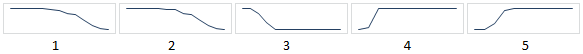
\includegraphics[scale=.9]{imgs/sparklines.png}
  \caption{1: Success Rate vs. Visitors, 2: Satisfaction
    vs. Visitors, 3: Satisfaction vs. Visitors,
    4: Success Rate and Satisfaction vs. Tolerance, 5: Tolerance vs. Success Rate and Satisfaction}
  \label{fig:sparklines}
\end{figure}

The success rate was 100\% for seasons with 5, 50, and 100
visitors (see \textbf{Figure \ref{fig:visitors-t2}}).
Once the number of visitors per season increased past 100, the
success rate began decreasing at an increasing rate.
Further increases in the number of visitors produced the following points
of interest:
\begin{itemize}
\item The success rate dropped from 100\% to 91\% between 100 and 300 visitors.
\item By 500 visitors, the success rate had fallen to below 25\%.
\item At 600 visitors the success rate appears to level off, asymptotically,
between zero and 5\%.
\end{itemize}
These values seem to follow an inverse of the problem's solution space.

Similarly, the average satisfaction of the visitors decreased with an increase in the
number of visitors (\textbf{Figure~\ref{fig:sparklines} Spark 2}).
Once the number of visitors per season increased past 100, the
satisfaction score began decreasing at an increasing rate. Satisfaction dropped
from 97.9\% to 89.4\% between 100 and 300 campers, then from 89.4\%
to 24.5\% between 300 and 500 campers. For seasons with more
than 500 groups, satisfaction leveled off, appearing to have an
asymptote just above zero percent. The satisfaction for a season with 600 visitors
was 4.9\%.

For seasons with a  1-site tolerance, the effect of visitor size increased
(\textbf{Figure~\ref{fig:sparklines} Spark 3}). Both the
success rate and satisfaction of visitors decreased with just a visitor size of
only 50 people. The success rate dropped from 100\% to 96\%
when visitor sized increased from 5 to 50 visitors per season. By just 250
visitors, both the success rate and the satisfaction were zero percent.

The tolerance for which campsite visitors stayed at each night had a positive
effect on success rate of the scheduler and satisfaction of the visitors
(\textbf{Figure~\ref{fig:sparklines} Spark 4}).  We noted the following points
of interest:
\begin{itemize}
\item For seasons with
200 visitors, a tolerance of zero campsites had a success rate of 0\%
and satisfaction of zero percent.
\item Increasing the tolerance to one campsite
resulted in a success rate of 52\% and a satisfaction of 4.9\%.
\item Increasing the tolerance to two campsites had the greatest effect, raising
success rate to 97.8\% and satisfaction to 95.9\%.
\end{itemize}
With any greater tolerances, the success rate was 100\%, and the satisfaction
leveled off at 97.8\%.  These results for tolerance agree with the notion that
the additional variability allows for more successful schedules.

For seasons with 500 visitors, a greater tolerance was needed to achieve
similar results (\textbf{Figure~\ref{fig:sparklines} Spark 5}).
A tolerance of 0 campsites
had a success rate of 0; a tolerance of 1 campsite had a success rate of
only 2.6\%; 2 campsites, 28\%; 3 campsites, 90\%. The
success rate was only 100\% with a tolerance of greater than 4 campsites,
and the satisfaction was 98\%.

Assigning more visitors to motorboats (those that travel at 8 mph) was seen
to increase the success rate. For a homogeneous season of 8 mph visitors, the
success rate was 98.2\% and the satisfaction 74\%. As the number
of 4 mph boats increased, both success rate and satisfaction steadily decreased.
With half rowboats and half motorboats, the success rate was 92\% and
the satisfaction 72\%. With a 9:1 ratio of rowboats to motorboats, the
success rate of the season was only 89.9\%. However, there is a jump
in success rate to 99\% once all visitors are traveling at 4 mph. This
jump in successes is not accompanied by a jump in satisfaction; with all
rowboats, the satisfaction is only 70\%.  This sort of relationship
between the mix of craft type and success rate is somewhat
surprising, given that an even mix might make more sense.  At this time, we
have no clear explanation for such behavior.

\subsection{Analysis}
\label{sec:capacity}
As defined in our definitions section, carrying capacity is
the amount of visitors a river can see in a single
year while maintaining the likelihood that all visitors will be scheduled and
remain satisfied. With a
tolerance of 2 campsites (\textbf{Figure~\ref{fig:visitors-t2}}), we found
the river could manage 100 visitors per
season with a 100\% success rate and a satisfaction of at least 97\%.
It is worth noting that doubling the capacity to 200 visitors per
seasons yields a success rate of 99.5\% and a satisfaction still greater
than 97\%. Once the number of visitors per season increases past 200,
both success rate and tolerance begin to drop rapidly.
\begin{figure}[h]
  \centering
  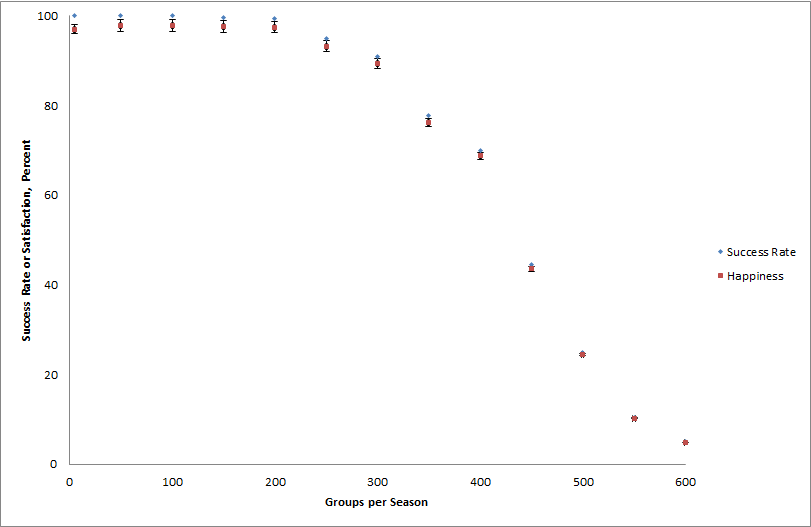
\includegraphics[scale=.6]{imgs/Graph_VistorsChanges_Tolerance2.png}
  \caption{Groups per Season vs. Success Rate and Satisfaction with Tolerance 2}
  \label{fig:visitors-t2}
\end{figure}
With a tolerance of 1 campsite, we found the river could only manage about
five visitors per season with a success rating of 100\%. The average
satisfaction of these visitors is 97.7\%. After the number of visitors per
season increases above 50, both satisfaction and success rate begin dropping
rapidly as seen in \textbf{Figure \ref{fig:visitors-t1}}.
\begin{figure}[h]
  \centering
  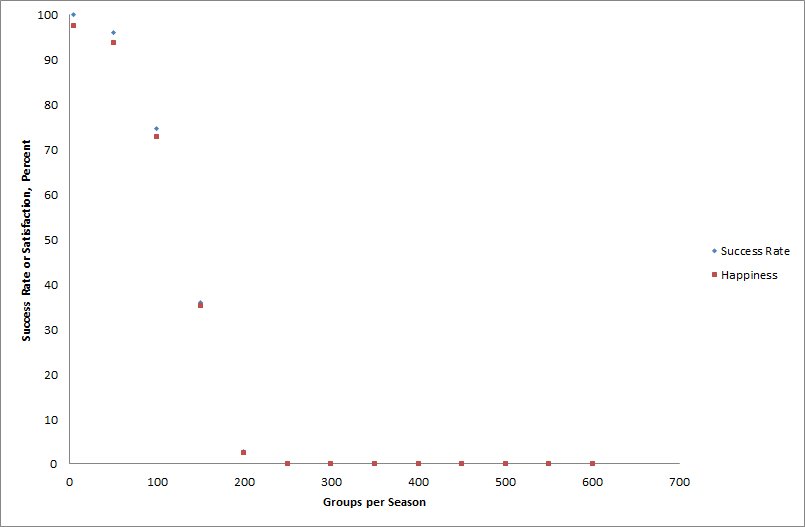
\includegraphics[scale=.6]{imgs/Graph_VistorsChanges_Tolerance1.png}
  \caption{Groups per Season vs. Success Rate and Satisfaction with Tolerance 1}
  \label{fig:visitors-t1}
\end{figure}

Is our value of 300 visitors, which was reasonably successful and maximal,
realistic?  Assuming that it is possible to have 60 individuals in a visitor
group, we find that our model allows for 18,000 people in a season to travel
down the Big Long River.  Our sources suggest this is realistic for
comparable rivers (i.e. the Colorado River)\cite{ColoradoRiverPaper}.

\section{Final Thoughts}
\label{sec:conclusions}
\subsection{Advantages to the Approach}
\label{sec:pros}
Throughout, we have seen that a constraint satisfaction approach to scheduling
visitors to a river is a natural fit.  This approach allows for a logical
approach to the scheduling process, and for fairly quick solutions.  In most
cases, solutions were found on mid-grade hardware in less than ten minutes.
We also found that the structure of our solution in both code and at a
higher level lent itself well to the adjustment of any number of parameters.
Moreover, there exists a great deal of flexibility once one begins to define
``fuzzy values'' that we can assign to the variables.  Given more time,
extending the model with these fuzzy values would likely lead to better
assignments and even more interesting results.

\subsection{Detractors from the Approach}
\label{sec:cons}
In our assumptions (\textbf{Section \ref{sec:assumptions}}) we note that the
visitors are basically perfect.  This, of course, is not true.  Due either to 
inclement weather, rudeness, or physical constraints we can not expect this 
behavior.  It is not immediately apparent
how to deal with this shortcoming other than simply accepting all variables 
can not be accounted for.  Padding the schedules with ``free days'' on
which any amount of travel lag may be recuperated.

The use of a consistent river in our model is less detrimental to the
overall performance and accuracy.  A realistic river would include areas
where passing other groups is impossible, visitors travel faster or slower,
and the potential for divisions of the river.  These could all be built in
as constraints on the campsites and their assignment to visitors.  Should
we have more time, this would likely be incorporated into the model.


\subsection{Future Extensions}
\label{sec:extensions}
Given more time there are several additions that would improve the technical
and practical performance of the model:
\begin{itemize}
\item The addition of a filtering technique to detect early failure in the
backtracking search.  This is often performed as what is called
``arc-consistency''.  Regretfully, it is difficult to implement for our
n-ary constraints.
\item Utilizing a fuzzy constraint for departure days would allow groups
to have a window in which they might leave.  This is likely to increase the
number of possible visitors, considering that it is nearly a direct analog
to tolerance.
\item The schedule might be modified to include days of rest for campsites
on a rotating basis.  This would not aid in adding more visitors (in fact it
would decrease the success rate), but it would assist in land management
practices and encourage a healthy use of the river ecosystem.
\end{itemize}


\subsection{Final Recommendations}
\label{sec:final}
Designating an exact number of visitors to raft down a river each year is
a complex problem that may not have only one solution. Managers will need
to be assertive in designating a tolerance, allotting departure days and
boat types to visitors, and instructing visitors to follow their schedules
carefully. Given certain parameters, however, we recommend a tolerance of
2 campsites, and about 300 visitors per season. Depending upon the current
number of visitors each season, $X$, \textbf{this would mean increasing the number
of visitors by 300-X}.  Note that those 300 visitors may be $groups$, not
necessarily individuals.  A tolerance of 2 campsites
permits a large number of visitors per season while maintaining acceptable
visitor satisfaction. Any greater tolerance would create a sharp decrease
in satisfaction as visitors are forced to travel unfortunate distances; any
smaller tolerance greatly decreases the chance of a successful schedule for
any large number of visitors. Any more than 300 visitors is likely to drop
both the chance of a successful season and the satisfaction of visitors.


\newpage


\bibliographystyle{amsplain}
\bibliography{mcm-2012-paper.bib}

\end{document}
